\section{ПРОЕКТИРОВАНИЕ И РАЗРАБОТКА}

\subsection{Выбор программных средств для реализации базы данных}

Выбор программных средств играет большое значение для проектируемой базы данных, поскольку определенные на этом этапе программные продукты, средства разработки и технологии непосредственным образом окажут влияние на распространение разработанной продукта: чем более распространенными будут используемые при разработке и требуемые для функционирования базы данных технологии, тем шире круг потенциальных потребителей, имеющих возможность ей воспользоваться. Кроме того, выбор среды разработки непосредственно влияет на стоимость и простоту процесса разработки в целом.

База данных «onmp» является реляционной. Реляционная база данных представляет собой набор таблиц, однако достаточно часто в состав базы данных входят и другие элементы, позволяющие дополнительно влиять на организацию и структуру данных в соответствии с определенным набором требований.

Создание и развитие динамических веб-страниц требует использования различных технологий. Разработка динамических веб-страниц включает три основных компонента: веб-сервер, язык программирования сценариев, исполняемых на стороне сервера, и базу данных.

Язык структурированных запросов (Structured Query Language, SQL) – самый распространенный язык, предназначенный для записи, извлечения, обновления и удаления информации в системах управления реляционными базами данных.

PostgreSQL (полное название «PostgreSQL: The world's most advanced open source relational database») - это мощная объектно-реляционная система управления базами данных (СУБД), которая поддерживает SQL-запросы и соответствует многим стандартам ANSI SQL. PostgreSQL является свободным и открытым программным обеспечением, доступным для использования и модификации бесплатно.

PostgreSQL обладает рядом преимуществ по сравнению с другими СУБД \cite{book2, book3} :

\begin{itemize}
    \item надежность и целостность данных: PostgreSQL имеет высокую степень надежности и обеспечивает высокую степень целостности данных благодаря поддержке транзакций, атомарности, согласованности и изоляции (ACID);
    \item безопасность: PostgreSQL обеспечивает множество функций безопасности, включая возможность управления правами доступа на уровне таблиц, столбцов, функций и процедур, проверку подлинности и защиту от SQL-инъекций;
    \item масштабируемость: PostgreSQL обладает высокой степенью масштабируемости и может обрабатывать большие объемы данных. Он поддерживает репликацию данных и многоуровневую архитектуру серверов;
    \item поддержка SQL: PostgreSQL поддерживает стандарт SQL и соответствует многим стандартам ANSI SQL, что облегчает разработку и поддержку приложений;
    \item расширяемость: PostgreSQL поддерживает расширения, которые позволяют разработчикам создавать свои собственные функции, типы данных и языки программирования, расширяя тем самым функциональность базы данных;
    \item мощный функционал: PostgreSQL имеет широкий функционал, включая поддержку полнотекстового поиска, гео-пространственных запросов, JSON- и XML-обработки, а также многопоточности;
    \item открытость: PostgreSQL является свободным и открытым программным обеспечением, доступным для использования и модификации бесплатно, что обеспечивает независимость от поставщика и поддержку со стороны большого сообщества разработчиков и пользователей.
\end{itemize}



\subsection{Проектирование базы данных}

Проектирование базы данных для любой автоматизированной системы разделяется на следующие этапы \cite{book5}:

\begin{itemize}
    \item определение требований к базе данных;
    \item концептуальное проектирование базы данных;
    \item выбор средств реализации базы данных;
    \item логическое проектирование;
    \item физическое проектирование.
\end{itemize}

Объекты, которые хранятся в базе данных, имеют некую логическую структуру, то есть описываются некоторой моделью представления данных. К числу классических моделей относят следующие: иерархическая, сетевая и реляционная.

Иерархическая модель представляет собой упорядоченную совокупность данных, организованных в виде дерева, где каждый узел содержит записи данных. Тип «дерево» является составным, состоящим из подтипов (поддеревьев), которые также являются типом "дерево". Каждый тип "дерево" состоит из одного корневого типа и упорядоченного набора подчиненных типов, устанавливая связь «предок-потомок».

Сетевая модель отображает различные взаимосвязи данных в произвольном графе и обобщает иерархическую модель данных. Она использует два типа данных: записи и связи. Связь определяется между двумя типами записей - предком и потомком. В отличие от иерархической модели, где потомок имеет только одного предка, здесь потомок может иметь произвольное число предков.

Реляционная модель основывается на понятии отношений и представляет собой множество элементов, называемых кортежами. Отношение часто представляется в виде двумерной таблицы. Каждая строка таблицы имеет одинаковую структуру и состоит из полей. Строкам соответствуют кортежи, а столбцам - атрибуты. Реляционная модель удобна для описания простых связей между объектами, где каждому объекту соответствует строка таблицы. Если требуется описать более сложные логические структуры данных, часто используют связывание нескольких таблиц.

Для реализации данной медицинской информационной системы будем использовать реляционную модель.

Концептуальная модель базы данных - это наглядная диаграмма, которая использует стандартные обозначения и детально показывает связи между объектами и их характеристиками. Концептуальная модель создается для последующего проектирования базы данных и ее преобразования, например, в реляционную базу данных. В концептуальной модели визуально отображаются связи между объектами данных и их характеристиками \cite{online4}.

ER-модель – модель данных, позволяющая описывать концептуальные схемы на основе диаграмм сущность-связь (ER-диаграмм).

Модель базы данных описывают с помощью одной или нескольких ER- диаграмм, содержащих сущности, атрибуты и связи.

Сущность определяется как объект, событие или концепция, информация о котором должна сохраниться. Сущности имеют наименование, несущее четкое смысловое значение. Каждый экземпляр сущности на диаграмме уникален.

Атрибут хранит информацию об определенном свойстве сущности и имеет четкое смысловое значение. Атрибут или группа атрибутов, которые однозначно идентифицируют экземпляры сущности, называются первичным ключом (англ. primary key).

Связь описывает логическое соотношение между сущностями. Связь сущности с другими сущностями определяет ее тип: различают два типа сущностей – зависимые и независимые.

Можно установить следующие связи между сущностями: идентифицирующая связь «Один–ко–Многим», связь «Многие–ко–Многим», неидентифицирующая связь «Один–ко–Многим» и связь «Один–к–Одному».

Связь «Многие–ко–Многим» существует только на логическом уровне. При переходе на физический уровень это отношение должно быть преобразовано за счет добавления новой зависимой сущности, связанной идентифицирующими связями «Один–ко–Многим» с сущностями, находящимися в исходном отношении.

Сущности, имеющие связь «Один–к–Одному», можно объединить в одну. При физической реализации базы данных две таблицы могут использоваться вместо одной по соображениям конфиденциальности, для удобства, для экономии дискового пространства, из семантических соображений.

Идентифицирующая связь устанавливается между независимой и зависимой сущностями, при этом зависимая сущность не может существовать самостоятельно - экземпляр зависимой сущности определяется только через отношение к сущности, которая его идентифицирует. При установлении идентифицирующей связи атрибуты первичного ключа родительской сущности автоматически переносятся в состав ключевых атрибутов дочерней сущности.  В дочерней сущности новые атрибуты помечаются как внешний ключ. В случае неидентифицирующей связи внешний ключ не входит в состав первичного ключа дочерней сущности.



\subsection{Проектирование логических моделей данных}

Проектирование модели данных состоит из двух уровней представления данных - логического и физического. Такое разделение на модели позволяет разделять задачу на более мелкие элементы.

Логический уровень – это некоторая абстрактная модель данных, позволяющая описать исследуемый объект, подчеркивая в нем необходимые свойства. Преимущество этого уровня заключается в том, что он является универсальным, поэтому реализовав его, можно создать БД, используя всевозможные для этого инструменты.

Различают три уровня логической модели, отличающихся по глубине представления информации о данных:

\begin{itemize}
    \item диаграмма сущность-связь (Entity Relationship Diagram, ERD);
    \item модель данных, основанная на ключах (Key Based model, KB);
    \item полная атрибутивная модель (Fully Attributed model, FA).
\end{itemize}

Диаграмма сущность-связь - этот тип логической модели используется при первоначальной разработке БД. Он позволяет описать основные объекты или процессы, необходимые для реализации в БД. Для этого вводятся 3 понятия: сущность, связь, атрибут. Сущность – это объект, находящийся в БД. Используя сущности, можно описать основные таблицы в будущей БД. Связь – это соединение или введение некоторого взаимодействия между сущностями. Если интерпретировать связь в БД, то связь выступает в роли внешних ключей. Атрибут – это ключевые элементы сущности, необходимые для его описания. В БД атрибут можно сравнить со столбцами, хранящимися в таблице. Этот тип моделирования позволяет опускать описание атрибутов, чтобы не загромождать диаграмму.

Модель данных, основанная на ключах - это дополненная ER-диаграмма. Ее главное отличие от первой: обязательное наличие некоторых атрибутов. Этими атрибутами являются первичные ключи, необходимые для соблюдения уникальности данных, и внешние ключи, обеспечивающие целостность данных. Стоит отметить, что внешние ключи никак не изображаются, они лишь являются следствием связей между сущностями. Причем внешний ключ находится у слабой сущности, а сам этот ключ ссылается на первичный ключ сильной сущности.

Первичные ключи принято обозначать как PK – Primary Key, графически они обозначаются двумя подчеркнутыми линиями, также допускается использование жирного шрифта. Внешние ключи принято обозначать как FK – Foreign Key, графически обозначаются одной подчеркнутой линией, допускается использование курсивного шрифта.

Полная атрибутивная модель - самая детализированная модель на логическом уровне. В ней исключается лишняя или дублирующая информация – этот процесс называется нормализацией БД. Помимо минимизации избыточной информации, в этой модели представляются все существующие сущности, связи и атрибуты.

Для построения полной атрибутивной модели используется IDEF1X нотация. В ней основными объектами также являются сущности, связи и атрибуты. Сущности называются в единственном числе и имеют четкое смысловое значение. Атрибуты должны именоваться в единственном числе и иметь четкое смысловое значение. Каждая связь должна именоваться глаголом или глагольной фразой, причем глагол ставится от 3 лица.

\subsection{Нормализация базы данных}

Для того, чтобы оптимизировать модель и избавиться от избыточных данных, проводят нормализацию данных. Нормализация – разбиение таблицы на две или более, обладающие лучшими свойствами при добавлении, изменении и удалении данных. Нормализация осуществляется с целью оптимизации объема БД и быстродействия запросов. Всего существует пять нормальных форм, но реально, на практике, используются лишь третья, а именно база данных в третьей нормальной форме (3НФ). Процесс нормализации отношений осуществляется пошагово и заключается в последовательном переводе отношения от первой нормальной формы к нормальным формам более высокого порядка. При этом каждая следующая нормальная форма сохраняет все свойства предыдущих.

Нужно проверить, находится ли полученная схема отношений в третьей нормальной форме (3НФ). Если схема отношений не находится в 3НФ, то ее нужно нормализовать для минимизации избыточности данных и устранения потенциальной противоречивости данных.

Отношение находится в первой нормальной форме (1НФ), если значения всех атрибутов атомарные, то есть значение атрибута не должно быть множеством или повторяющейся группой.

Отношение находится во второй нормальной форме (2НФ), если оно находится в 1НФ, и нет частичной функциональной зависимости неключевых атрибутов от ключа (зависимость не ключевых атрибутов от части ключа). Из схемы отношений видно, что ни один из неключевых атрибутов функционально полно не зависит от ключа, следовательно, схема отношений находится в 2НФ.

Отношение находится в 3НФ, если оно находится во 2НФ, и отсутствуют транзитивные зависимости неключевых атрибутов от ключа. Между атрибутами A и C есть транзитивная зависимость, если выполняется совокупность условий: если хотя бы одно из условий не выполняется, то транзитивной зависимости между атрибутами A, B, C нет. Причем атрибуты A, B, C могут быть составными \cite{online12}.

Анализируя атрибуты, можно сделать вывод, что транзитивная зависимость отсутствует, то есть отношение находится в 3НФ. Следовательно, все схемы отношений являются окончательными схемами отношений.

\subsection{Проектирование физических моделей данных}

В отличие от логической модели, физическая модель строится в зависимости от выбранной СУБД. Также этот вид модели позволяет напрямую создавать команды для системного каталога СУБД. Главное отличие физической от логической модели состоит в том, что в первой уделяется внимание на типы объектов. Так, атрибуты могут иметь разные форматы данных: например, числовой или строчный. Помимо формата данных, физическая модель допускает использование физических объектов СУБД: например, процедуры.

Различают два уровня физической модели:

\begin{itemize}
    \item трансформационная модель (Transformation Model);
    \item модель СУБД (DBMS Model).
\end{itemize}

Трансформационная модель содержит информацию для реализации отдельного проекта, который может быть частью общей ИС и описывать подмножество предметной области. Трансформационная модель позволяет проектировщикам и администраторам БД лучше представлять, какие объекты БД хранятся в словаре данных, и проверить, насколько физическая модель данных удовлетворяет требованиям к ИС.

Модель СУБД является точным описанием того, как выглядит будущая БД в системном каталоге СУБД. Именно эта модель физического уровня будет использоваться в данной работе, потому что она имеет практическое влияние.

Самым главным объектов в БД является таблица. Если интерпретировать физическую модель через логическую, то получим такой вывод, что таблицы являются сущностями, столбцы - атрибутами, а связи образуются через внешние ключи. Таблица содержит столбцы, именно поэтому им стоит уделить достойное внимание.

Первое свойство столбца, про которое стоит сказать, может ли оно принимать нулевые значения, в случае если может, нужно писать этому столбцу предложение «NULL», иначе «NOT NULL». Причем первичные ключи не могут быть нулевыми значениями, также не рекомендуется использовать «NULL» для внешних ключей. Второе свойство столбца есть сам формат данных, для целочисленных (причем 0 в старшем бите, не являющемся значимым) стоит использовать «INTEGER», для строковых значений можно использовать «VARCHAR(n)», а для использования даты применяется «DATE», а если нужна дата с временем, то «DATETIME» \cite{online5}.




\subsection{Готовые решения}

Проанализировав программные средства для реализации баз данных, рассмотрев все основные принципы построения столбцов, создания первичных и внешних ключей и нормализацию данных, приведем ER-диаграммы основных структур \cite{book4}.

Логично предположить, что для начала нам нужно будет создать аккаунт и пройти аутентификацию в приложении, пройдя верификацию по логину и паролю. Здесь возможно два исхода:

\begin{itemize}
    \item верификация прошла успешно;
    \item отказано в доступе.
\end{itemize}

Как уже говорилось раннее, у нас возможны некоторые роли:

\begin{itemize}
    \item администратор;
    \item пользователь.
\end{itemize}

В зависимости от этого у нас будут формироваться данные входа для разных ролей. Соответсвенно для этого нам нужно сделать структуру таблиц под эти требования. На рисунке~\ref{fig:fig01} показана ER-диаграмма организации структуры для хранения данных о пользователе с определенными правами, ролями и группами.

\begin{figure}
  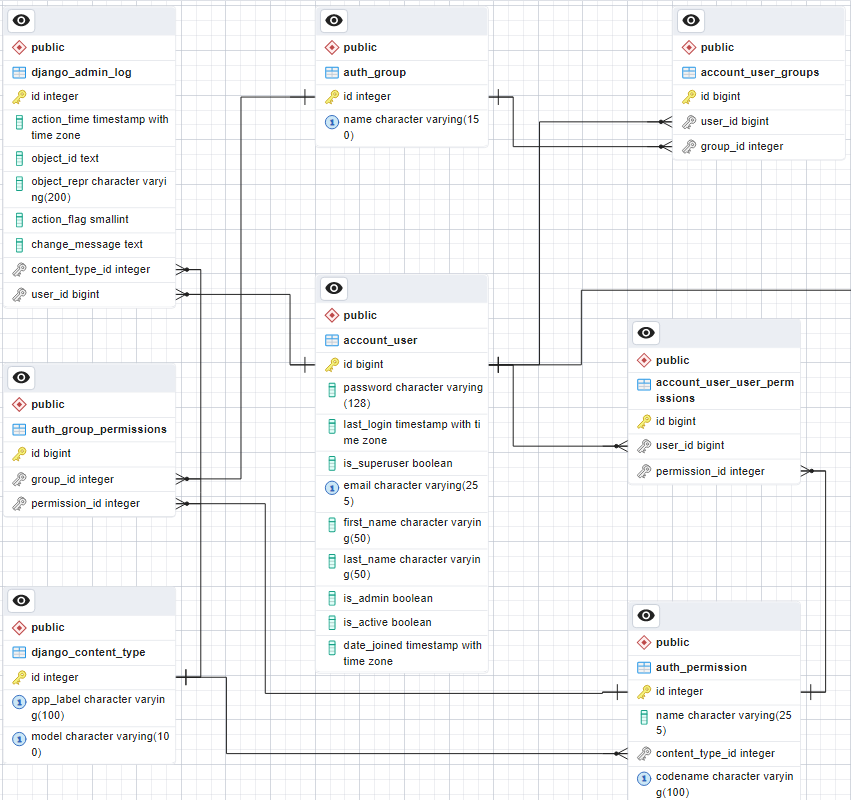
\includegraphics[scale=0.733]{inc/django}
  \caption{Данные пользователя с определенными правами, ролями и группами}
  \label{fig:fig01}
\end{figure}

Как можно заметить, на рисунке~\ref{fig:fig01} видна еще одна связь, которая уходит за пределы изображения. Это не случайно, сейчас объясним этот момент.

На рисунке~\ref{fig:fig02} показана ER-диаграмма организации структуры хранения данных для связи нашей БД с взаимодействиями на стороне back-end'а. Есть таблица, которая заполняется при первичной регистрации пользователя и служит для информации на стороне back-end'а. Кроме того, есть таблица пользователя, которая нужна только в БД и служит непосредственно для связи пользователя с медицинскими картами пациентов, которые заполняет медицинский работник при выезде.

\begin{figure}
  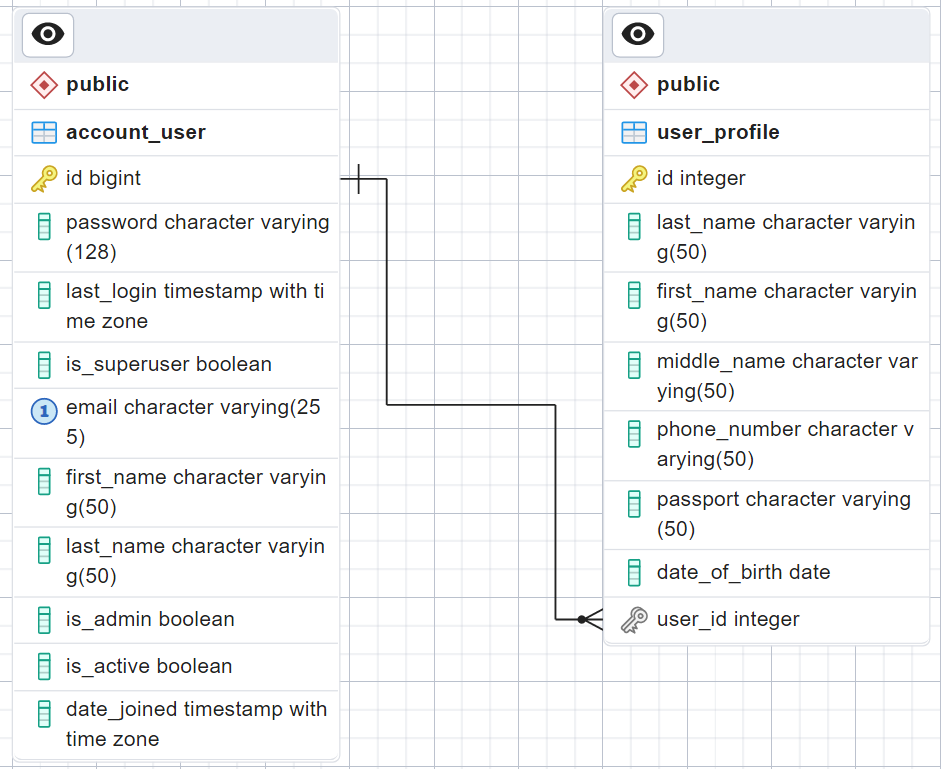
\includegraphics[scale=0.655]{inc/user_account_user_profile}
  \caption{Связи взаимодействия}
  \label{fig:fig02}
\end{figure}

На рисунке~\ref{fig:fig02} была схематично показана связь двух таблиц. Теперь приведем описание таблицы user\_profile и объясним ее назначение в нашей БД. На рисунке~\ref{fig:fig03} показана ER-диаграмма организации структуры хранения данных для пользователей нашего приложения.

\begin{figure}
  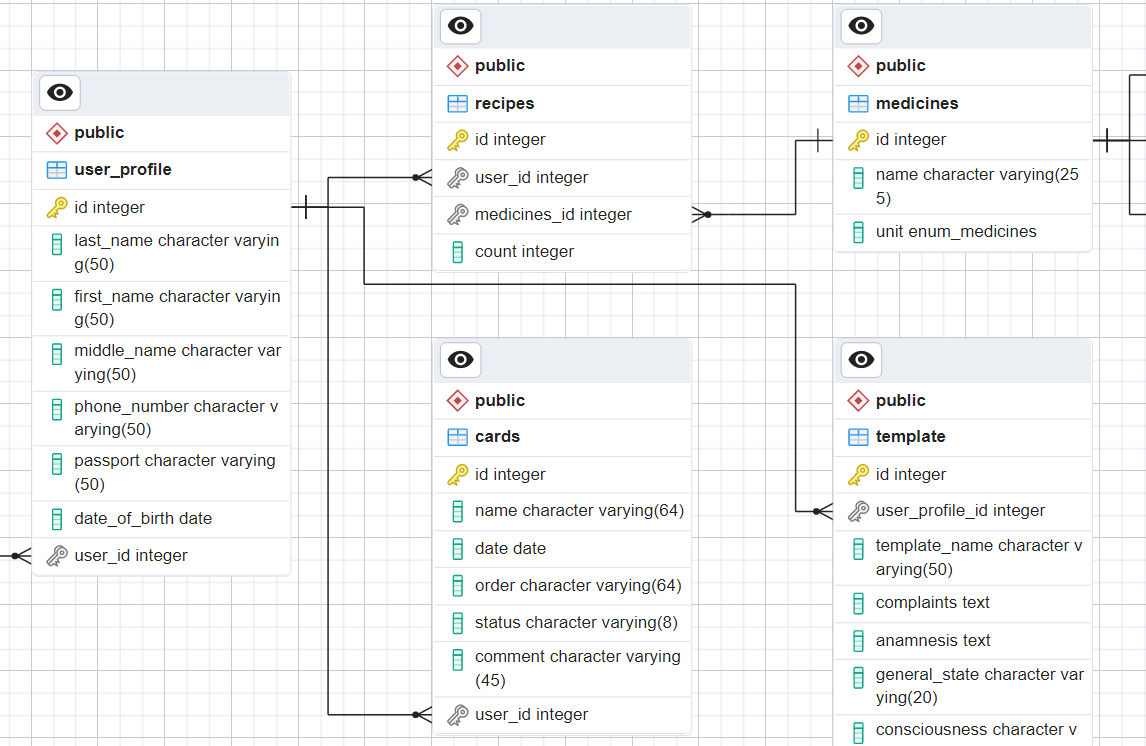
\includegraphics[scale=0.54]{inc/user_profile}
  \caption{Пользователь}
  \label{fig:fig03}
\end{figure}

Как можно заметить, в таблице medicines есть еще три связи, которые не попали на данный рисунок. Эти связи будут продемонстрированы на рисунке~\ref{fig:fig07}.

На рисунке~\ref{fig:fig04} показана ER-диаграмма организации структуры хранения данных полного взаимодействия с момента регистрации и аутентификации пользователя в приложении до связи определенного медицинского работника с шаблоном для заполнения медицинской карты при выезде к пациенту.

\begin{figure}
  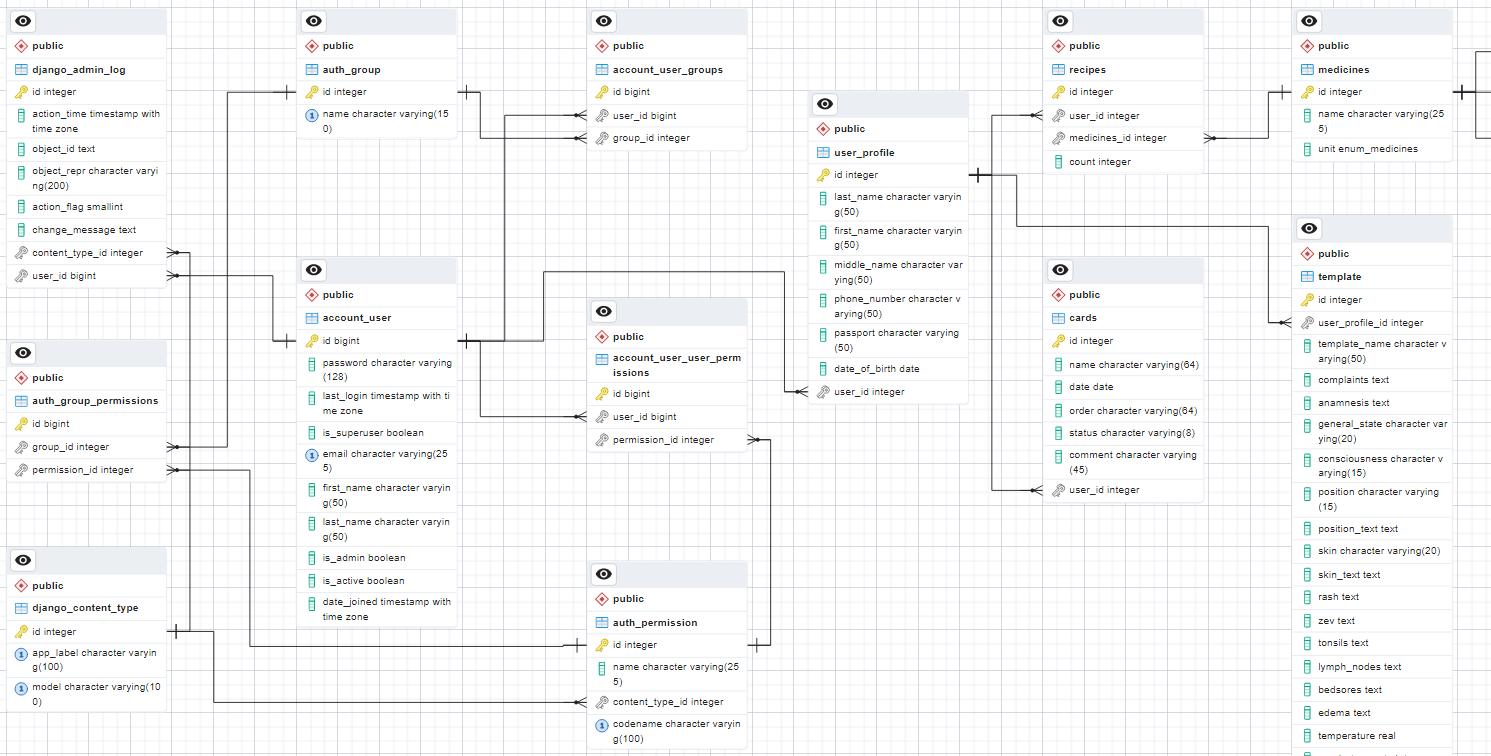
\includegraphics[scale=0.418]{inc/django_user_profile}
  \caption{Полная структура взаимодействия}
  \label{fig:fig04}
\end{figure}

На рисунке~\ref{fig:fig05} показана ER-диаграмма организации структуры хранения данных для диагнозов. Каждый диагноз относится к определённому направлению в медицине - так называемый тег. Каждый диагноз имеет свой определенный код МКБ. У диагноза есть свой определенный перечень оказания объема необходимой медицинской помощи и тактика выполнения действий. Кроме того, диагноз имеет свои так называемые формы(поддиагнозы) и относящийся уже к ним объем необходимой медицинской помощи.

\begin{figure}
  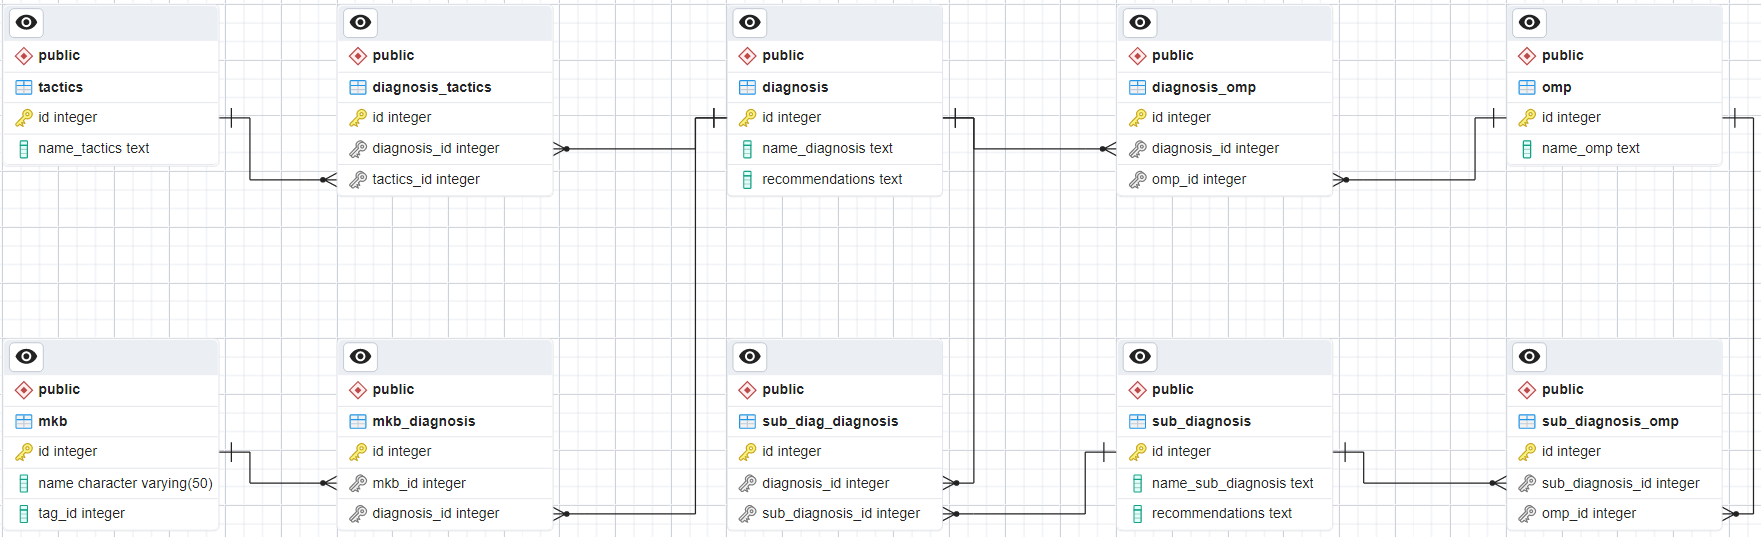
\includegraphics[scale=0.354]{inc/diagnosis}
  \caption{Диагнозы}
  \label{fig:fig05}
\end{figure}

На рисунке~\ref{fig:fig06} показана ER-диаграмма организации структуры хранения данных для заболеваний. Каждое заболевание относится к определённой категории в медицине - так называемый тег. У заболеваний есть свои определённые симптомы. Кроме того, заболевание имеет свой собственные формы и относящиеся уже к этой форме симптомы.

\begin{figure}
  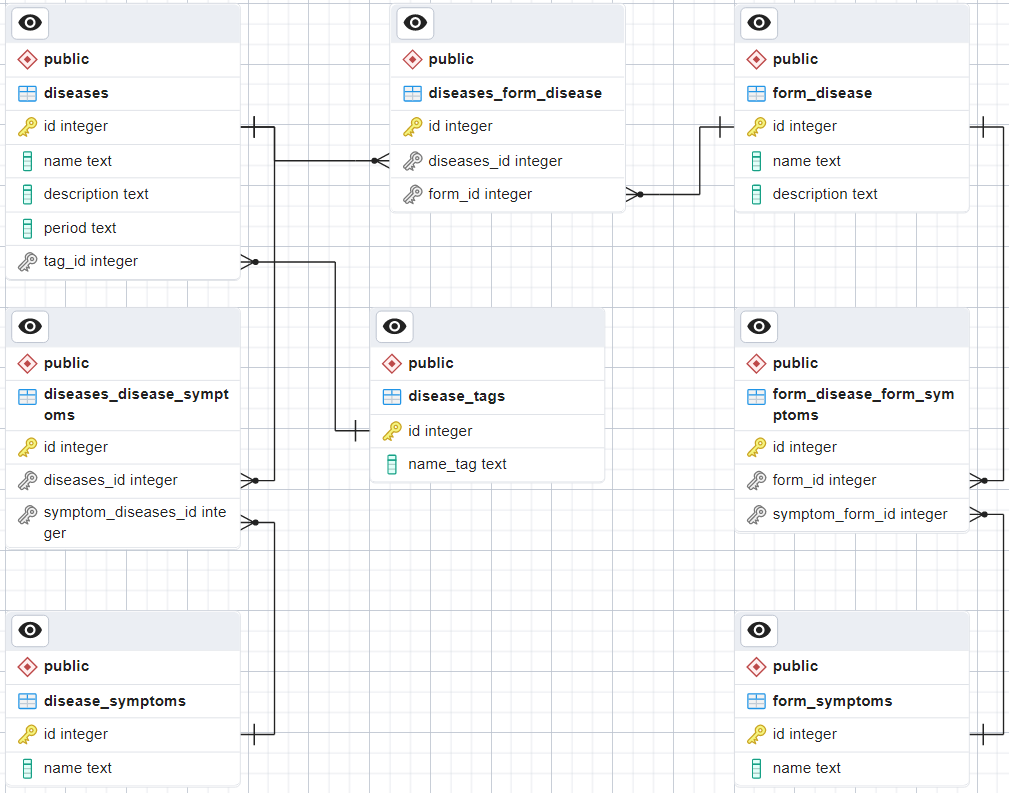
\includegraphics[scale=0.61]{inc/diseases}
  \caption{Заболевания}
  \label{fig:fig06}
\end{figure}

На рисунке~\ref{fig:fig07} показана ER-диаграмма организации структуры хранения данных для медикаментов. Каждый препарат имеет определенные противопоказания, взрослую и детскую дозировки, которые, в свою очередь зависят от конкретного диагноза.

\begin{figure}
  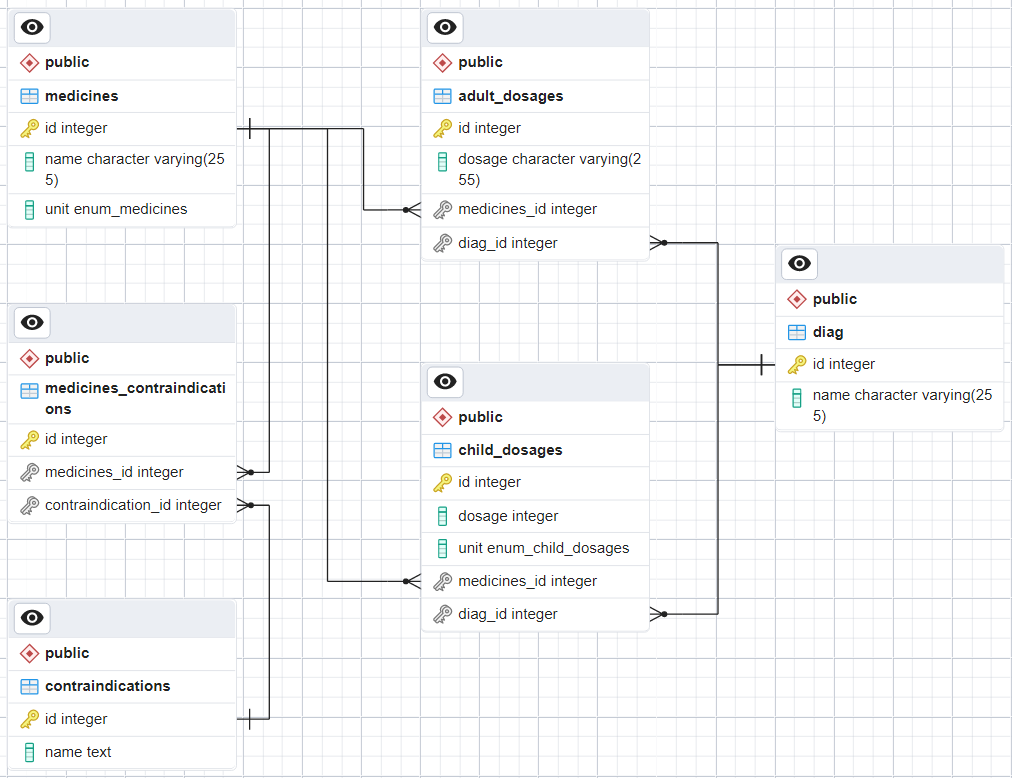
\includegraphics[scale=0.615]{inc/medicines}
  \caption{Медикаменты}
  \label{fig:fig07}
\end{figure}

Конечно, это не все таблицы, требуемые для функционала целого приложения. Медицинскому работнику иногда требуется какая-то незначительная вспомогательная информация и какой-то сложной организационной структуры эти таблицы не требуют. Вывод этих таблиц можно будет увидеть при выполнении запросов.

Таким образом, были объявлены основные таблицы БД, были рассмотрены столбцы, а именно проанализированы типы данных, а также определены ограничения для внесения конкретных значений. Этого достаточно, чтобы между таблицами сохранялась целостность данных, а вставка значений была корректной \cite{online1, online2, online3}.

Важно понимать, что перед внедрением базы данных необходимо провести тестирование и проверку ее функциональности, производительности и безопасности. Это поможет выявить потенциальные проблемы и ошибки, которые могут повлиять на работу системы. Регулярное тестирование после внедрения также является важной частью обслуживания базы данных.



\bigbreak
\textbf{Выводы по разделу}
\bigbreak

В этом разделе разбирались теоретические сведения, связанные с созданием БД. С помощью анализа организации и метода моделирования мы смогли решить задачи, связанные с определением предметной области ОНПМ и разработкой логических и физических моделей БД. На основе этих моделей были созданы таблицы в PostgreSQL, а для графического представления использовалось такое ПО как pgAdmin. Также была выполнена практическая задача, связанная с формированием системного каталога структуры БД.

Важно отметить, что разработка базы данных не является заключительным шагом. Необходимо предусмотреть систему поддержки и обслуживания, которая будет обеспечивать регулярные обновления базы данных, исправление ошибок, мониторинг производительности и резервное копирование данных. Регулярное техническое обслуживание поможет сохранить работоспособность и безопасность базы данных на протяжении всего ее существования \cite{online13}.